% Generated by Slides/extract_figures.py from Lecture3/lecture3.tex; do not edit.

    \pgfplotsset{hessplot/.style={x={(1.95cm,-0.65cm)}, y={(1.3cm,1.24cm)}, z={(0cm,0.98cm)}, axis lines=none, colormap/viridis}}
    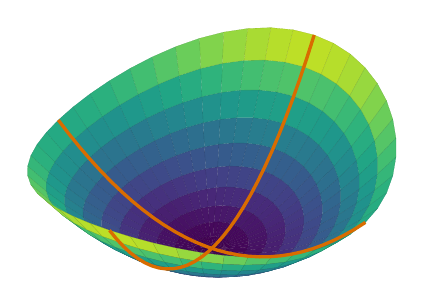
\begin{tikzpicture}
        \begin{axis}[hessplot]
            \addplot3[surf, shader=faceted, draw=black!25, line width=0.05pt, domain=0:1, y domain=0:360, samples=11, samples y=49, z buffer=sort] ({x*cos(y)}, {x*sin(y)}, {x^2*cos(y)^2 + 1.5*x^2*sin(y)^2});
            \addplot3[orange!85!black, very thick, domain=-1:1, samples y=0, samples=30] ({x}, {0}, {x^2});
            \addplot3[orange!85!black, very thick, domain=-1:1, samples y=0, samples=30] ({0}, {x}, {1.5*x^2});
        \end{axis}
    \end{tikzpicture}\hfill
    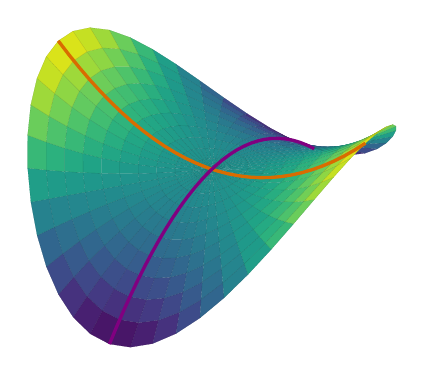
\begin{tikzpicture}
        \begin{axis}[hessplot]
            \addplot3[surf, shader=faceted, draw=black!25, line width=0.05pt, domain=0:1, y domain=0:360, samples=11, samples y=49, z buffer=sort] ({x*cos(y)}, {x*sin(y)}, {x^2*cos(y)^2 - x^2*sin(y)^2});
            \addplot3[orange!85!black, very thick, domain=-1:1, samples y=0, samples=30] ({x}, {0}, {x^2});
            \addplot3[violet, very thick, domain=-1:1, samples y=0, samples=30] ({0}, {x}, {-x^2});
        \end{axis}
    \end{tikzpicture}\hfill
    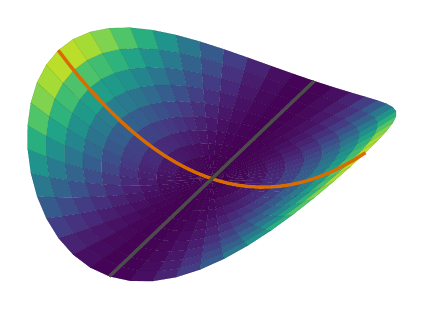
\begin{tikzpicture}
        \begin{axis}[hessplot]
            \addplot3[surf, shader=faceted, draw=black!25, line width=0.05pt, domain=0:1, y domain=0:360, samples=11, samples y=49, z buffer=sort] ({x*cos(y)}, {x*sin(y)}, {x^2*cos(y)^2});
            \addplot3[orange!85!black, very thick, domain=-1:1, samples y=0, samples=30] ({x}, {0}, {x^2});
            \addplot3[black!70, very thick, domain=-1:1, samples y=0, samples=30] ({0}, {x}, {0});
        \end{axis}
    \end{tikzpicture}
